%! Author = matteomagnini
%! Date = 05/03/25

%----------------------------------------------------------------------------------------
\chapter{NeSy AI for real world applications}
\label{ch:nesy-ai-for-real-world-applications}
\mtcaddchapter
\minitoc
%----------------------------------------------------------------------------------------

\section{Goals and challenges}\label{sec:nesy-ai-goals-and-challenges}

% \section{Applications}\label{sec:nesy-ai-applications}
%
We now present a selection of contributions about \gls{NeSy} application in real-world scenarios.
%
These works involve the use of both \gls{SKE} and \gls{SKI} methods, as well as traditional \gls{ML} models and the recent \glspl{LLM}.



\section{\Gls{SKE} for explainable nutritional recommenders}\label{sec:ske-for-explainable-nutritional-recommenders}
%
``Symbolic knowledge extraction for explainable nutritional recommenders''~\cite{DBLP:journals/cmpb/MagniniCCAO23}, published on the Journal of Computer Methods and Programs in Biomedicine, presents a novel nutritional recommender system that leverages \gls{SKE}.


\subsection{Nutritional recommender systems}\label{subsec:nutritional-recommender-systems}

Eating habits significantly impact the well-being of individuals across all age groups, highlighting the importance of developing nutritional \glspl{RS}~\cite{EspinHN2016,Cioara2018,Shandilya2022}.
%
These systems address diverse user needs, including diet programs, chronic disease management, treatment for critically ill patients, allergies, lifestyle choices (e.g., sporty, vegetarian, organic, halal), and physical activity levels~\cite{Saiz2021,Hezarjaribi2019,AgapitoSCCLGPFC2018,FraserT1990,Tran2018}.
%
User preferences are represented either by expert knowledge, such as daily nutritional intake limits based on physical activity levels, or by user feedback, such as reviews on recipes~\cite{10.1145/3418211}.
%
Recommendation items, such as food, recipes, and meals, are represented in terms of their attributes, including cuisine, category, cooking style, preparation time, and nutritional levels.
%
The complexity of nutritional \glspl{RS} arises from the combination of multiple ingredients to form recipes and the diverse attributes influencing user preferences.

Classical approaches to nutritional recommendation rely on content based and collaborative filtering methods, which derive user profiles from past activities, such as ratings, clicks, reviews, and browsing history~\cite{Min2020}.
%
Recent advancements leverage \gls{ML} techniques, including question answering over knowledge bases, recipe retrieval from visual records of ingredients, and learning recipe representations from multi-modal data~\cite{Forbes2011,Bianchini2017,Freyne2010,Chen2021,Tian2022}.
%
Despite the availability of recipes online, many are suboptimal in terms of health~\cite{Trattner2017a}.
%
Recent studies aim to promote healthy eating by incorporating healthiness indicators into recommendations or enhancing the visual appeal of food~\cite{Saiz2021,10.1145/3418211}.
%
Providing explanations for recommendations improves user trust and acceptance, as transparent systems are preferred over black-box models~\cite{Anjomshoae2019}.
%
Explainable approaches, such as explanation ontologies and multi-agent architectures, have been proposed to enhance both personalisation and explainability in nutritional \glspl{RS}~\cite{DBLP:conf/icde/PadhiarSCGM21,Yera2022,expectation-extraamas2021}.

\subsection{Methodology}\label{subsec:methodology}
%
\begin{figure}
  \centering
  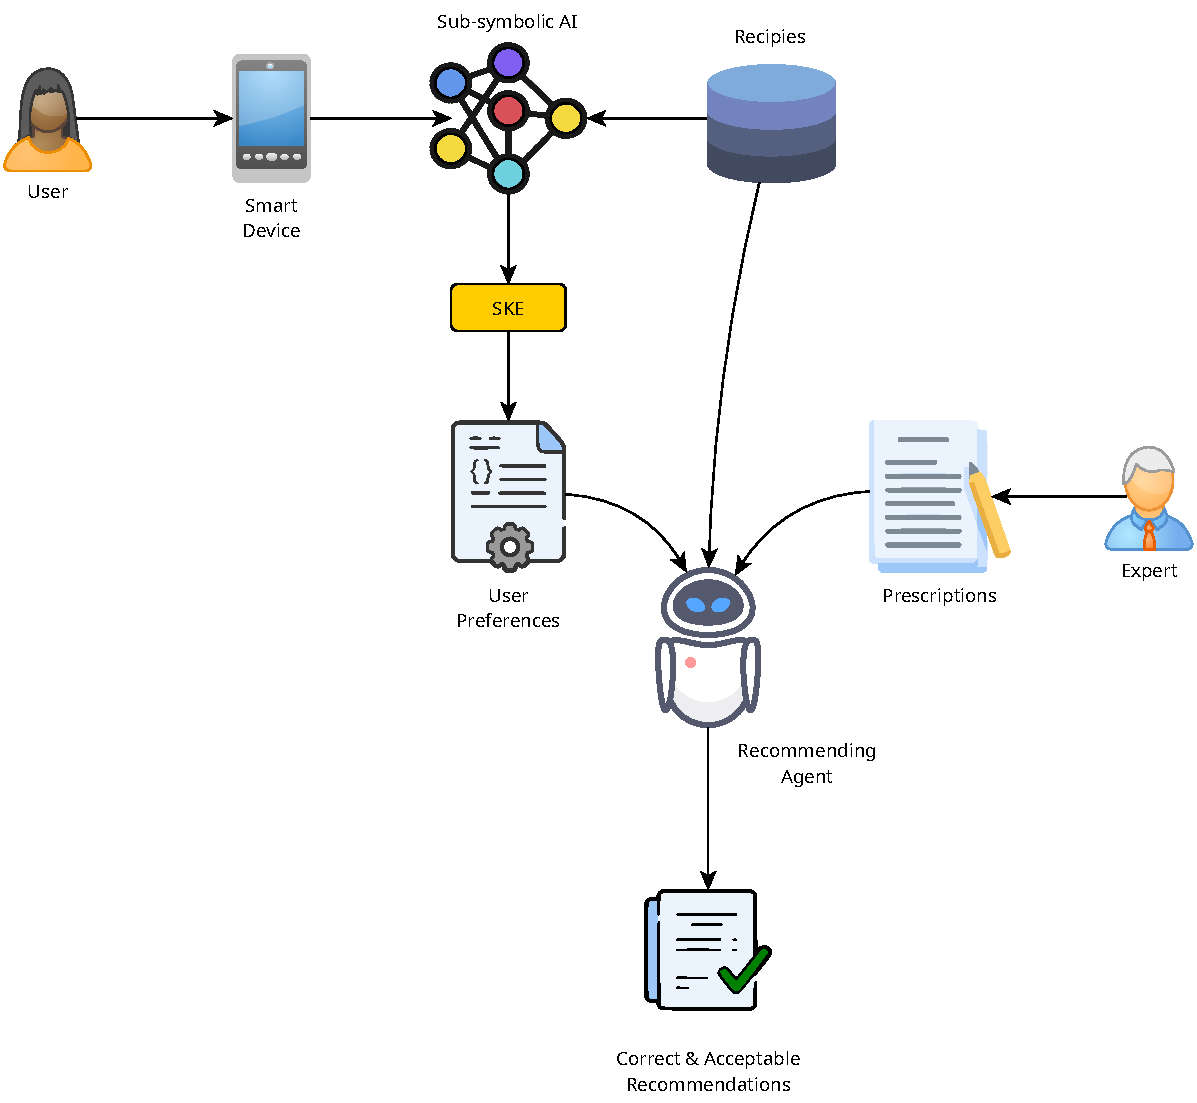
\includegraphics[width=\textwidth]{figures/ske-recommender-workflow}
  \caption{
    Data-flow perspective of a nutritional \gls{RS}.
    %
    The user interacts -- via some smart/wearable device -- with a sub-symbolic AI predictor, continuously trained to predict whether the user likes a given recipe or not.
    %
    A knowledge base is then extracted from the predictor, representing the user's preferences in a human-interpretable logic form.
    %
    Dietary prescriptions -- provided by human experts -- are transformed into the same logic form.
    %
    Conversely, databases providing information about recipies -- there including ingredients and their nutrients -- are assumed to be remotely available via the Internet.
    %
    Finally, the recommending agent exploits a logic engine, combining all such information into recommendations which are simultaneously correct (w.r.t.\ experts prescriptions), acceptable (w.r.t.\ users' preferences), and explainable.
  }
  \label{fig:ske-recommender-workflow}
\end{figure}

We propose a general architecture for nutritional \glspl{RS}, designed to provide personalised dietary recommendations aligned with specific user goals.
%
\Cref{fig:ske-recommender-workflow} illustrates the main components and data flow within the system.
%
The proposed architecture personalises dietary recommendations by identifying recipes that lie at the intersection of user preferences and expert prescriptions.
%
This process relies on three distinct sources of information:
\begin{inlinelist}
    \item the user,
    \item the nutrition expert, and
    \item the recipe database.
\end{inlinelist}
%
Users provide their preferences, which are learned adaptively by a sub-symbolic \gls{ML} predictor.
%
Nutrition experts translate dietary goals into structured prescriptions, which define patterns of recipes suitable for achieving these goals.
%
The recipe database stores information about recipes, their ingredients, and corresponding nutrients, enabling the agent to propose admissible options.
%
Recommendations are generated by combining these sources using a logic-based approach, ensuring alignment with both user preferences and expert prescriptions.
%
In the following sections, we detail how preferences, prescriptions, and recipes are represented and manipulated within the system.
%
We also describe the algorithmic process for producing recommendations and discuss its underlying assumptions.


\paragraph{Recipes}\label{par:recipes}
%
Our architecture identifies three key data types: recipes, ingredients, and nutrients.
%
Recipes are composed of ingredients, which in turn contain various nutrients.
%
Each data type is named, meaning recipes, ingredients, and nutrients are uniquely identified by their names.
%
The architecture does not track the preparation process of meals but focuses on the nominal composition of ingredients and their quantities.
%
By analyzing the composition of ingredients in terms of nutrients, the system computes the overall nutritional values of recipes.
%
The recipes' database is responsible for storing information about recipes, ingredients, and nutrients.
%
It supports several types of queries, such as:
%
\begin{itemize}
  \item Selecting recipes based on their ingredients or nutrients.
  %
  \item Filtering recipes by specific quantities of ingredients or nutrients.
  %
  \item Retrieving the ingredients or nutrients associated with a recipe.
  %
  \item Clustering recipes with similar nutritional profiles.
\end{itemize}
%
These queries are essential for the recommender agent's functionality.


\paragraph{Users' Preferences}\label{par:users-preferences}
%
User preferences are represented sub-symbolically using a \gls{ML} predictor.
%
This predictor learns user tastes adaptively from data, which includes information about recipes the user likes or dislikes.
%
Preferences are modeled as a function:
%
\begin{equation}
  \label{eq:users-preferences}
  \text{appreciation}: R \to \mathbb{R}
\end{equation}
%
where \( R \) is the set of admissible recipes, and the output is an appreciation score.
%
Positive values indicate liking, negative values indicate dislike, and zero represents neutrality.
%
The appreciation score encapsulates user opinions, including factors such as taste, allergies, and ethical beliefs.
%
Data is collected during user interactions, often via smart or wearable devices, and used to train the \gls{ML} predictor.
%
The learning process is continual, ensuring the system adapts to evolving user preferences.
%
The sub-symbolic approach enables generalization of user data while leveraging information from the recipes' database.


\paragraph{Dietary Prescriptions}\label{par:dietary-prescriptions}
%
Dietary prescriptions are structured representations of what a user should eat and when, to achieve specific goals.
%
They are typically created by nutrition experts based on the user's physiological characteristics and expert knowledge.
%
Prescriptions consist of two components:
%
\begin{itemize}
  \item The \emph{what} component specifies ingredients or nutrients and their quantities for each meal.
  %
  \item The \emph{when} component indicates the time of consumption (e.g., breakfast, lunch, dinner).
\end{itemize}
%
The goal reflects the expected long-term effect on the user's health, though it may not be explicitly stated.
%
Prescriptions are often provided in quasi-natural language or tabular formats.
%
In tabular form, each cell corresponds to a specific time and meal, listing the recommended nutrients or ingredients.
%
Users may construct recipes based on these suggestions unless a nutritional \gls{RS} is available.
%
For simplicity, we focus on a single prescription for a given time \( t \), expressed as logic formulas.
%
These formulas define the properties a meal should have to align with dietary goals.
%
Details on the use of logic formulas for dietary prescriptions are provided in the next subsection.


\paragraph{The role of logic formulas}\label{par:the-role-of-logic-formulas}

The proposed architecture utilizes Horn clauses to represent both user preferences and expert prescriptions.
%
Horn logic provides a clear and computationally tractable framework for expressing dietary prescriptions.
%
These formulas can be manually written by humans or algorithmically generated, enabling their use in \glspl{RS} for dietary recommendations.

%
Expert prescriptions at time \( t \) are defined as a set of Horn clauses describing the \texttt{should\_eat/1} predicate.
%
This predicate specifies the recipes that the user should consume, based on admissible or forbidden ingredients and nutrients.
%
Two auxiliary predicates, \texttt{has/2} and \texttt{has\_no/2}, are used to assert the presence or absence of specific ingredients or nutrients.
%
Groups of ingredients or nutrients can also be defined using unary predicates, such as \texttt{vegetable/1}.

%
For example, a dietary prescription for Monday lunch can be expressed as:
%
\begin{align*}
  \begin{array}{rcl}
    \texttt{should\_eat}(R) &\leftarrow& \texttt{has}(R, \texttt{rice}) \land \texttt{has}(R, \texttt{chicken}) \\
                            &\land& \texttt{has\_no}(R, \texttt{salt}) \\
                            &\land& \texttt{has}(R, X) \land \texttt{vegetable}(X)
  \end{array}
\end{align*}
%
indicating that the user should consume recipes containing rice, chicken, and any vegetable, but excluding salt.

%
To ensure self-containment, additional rules must define the semantics of predicates such as \texttt{has/2}, \texttt{has\_no/2}, and \texttt{vegetable/1}.
%
For brevity, these definitions are omitted here.

%
Alternative encodings, such as including a predicate \texttt{quantity(X, Q)} to specify the quantity \( Q \) of ingredient \( X \), are possible but do not alter the core contribution.
%
Thus, simpler syntactic choices are preferred.

%
User preferences can also be represented as Horn clauses, defining the \texttt{likes/1} predicate.
%
These clauses may use the same auxiliary predicates (\texttt{has/2}, \texttt{has\_no/2}) and custom predicates for grouping ingredients or nutrients.

%
Consider the following example:
%
\begin{align*}
  \begin{array}{rcl}
    \texttt{likes}(R) &\leftarrow& \texttt{has}(R, \texttt{rice}) \land \texttt{has}(R, \texttt{chicken}) \\
                      &\land& \texttt{has\_no}(R, \texttt{broccoli}) \land \texttt{has}(R, \texttt{peas}) \\
    \texttt{vegetable}(\texttt{peas}) &\leftarrow \\
    \texttt{vegetable}(\texttt{broccoli}) &\leftarrow \\
    \texttt{has}(\texttt{paella}, \texttt{rice}) &\leftarrow \\
    \texttt{has}(\texttt{paella}, \texttt{chicken}) &\leftarrow \\
    \texttt{has}(\texttt{paella}, \texttt{peas}) &\leftarrow \\
    \texttt{has}(\texttt{paella}, \texttt{seafood}) &\leftarrow
  \end{array}
\end{align*}
%
This example states that the user likes recipes containing rice, chicken, and peas (e.g., paella), but dislikes broccoli.
%
It also defines peas and broccoli as vegetables and specifies the composition of paella.

%
When both prescriptions and preferences are expressed as Horn clauses, their intersection can be computed using logic resolution.
%
This involves proving the query:
%
\begin{equation}
    \label{eq:intersection-prescriptions-preferences}
    \texttt{likes}(R) \land \texttt{should\_eat}(R)
\end{equation}
%
against the merged clause set of prescriptions and preferences.
%
The logic solver identifies recipes \( R \) that satisfy both conditions or determines that no such recipes exist.

%
For instance, testing the query above against the merged clauses from the examples provided yields \( R = \texttt{paella} \).
%
This result is denoted as:
%
\begin{equation}
  \label{eq:intersection-prescriptions-preferences-final}
  (3) \cup (4) \models \texttt{likes}(\texttt{paella}) \land \texttt{should\_eat}(\texttt{paella})
\end{equation}


\paragraph{The role of \gls{SKE}}\label{par:the-role-of-ske}
%
Our proposed architecture requires both user preferences and expert prescriptions to be expressed as sets of Horn clauses.
%
This representation enables the use of logic resolution to construct recommendations.
%
Expert prescriptions are typically provided in formats, such as timetables of suggested recipes, that can be directly expressed or automatically converted into Horn clauses~\cite{DBLP:journals/jcss/Makowsky87}.
%
This assumption aligns with current practices in dietary planning.
%
In contrast, user preferences are modeled using sub-symbolic predictors, such as trained \glspl{NN}, which adaptively learn preferences from data.
%
While sub-symbolic representations are effective for capturing dynamic user preferences, they are incompatible with direct logic resolution.
%
To bridge this gap, the architecture incorporates a \gls{SKE} step.
%
This step extracts symbolic knowledge in the form of Horn clauses from the sub-symbolic predictor trained to model user preferences.
%
The choice of \gls{SKE} algorithm is left to the implementer, allowing flexibility to select the most suitable method for their application.
%
However, the extraction process must produce Horn clauses to ensure compatibility with the logic-based recommendation framework.
%
This approach combines the adaptability of sub-symbolic models with the interpretability and computational efficiency of symbolic reasoning.


\subsection{Validation}\label{subsec:validation-ske-nutrition}
%
To validate the proposed architecture, we conducted a series of experiments to assess its effectiveness in nutritional \glspl{RS}.
%
The source code and instructions for reproducing these experiments are public available\footnote{\url{https://github.com/pikalab-unibo/mccao-cmpb-experiments-2022}}
%
The experiments involved four main steps:
%
\begin{enumerate}
  \item Generating synthetic datasets to simulate a single user's food preferences.
  %
  \item Training a \gls{ML} predictor, specifically a neural network, to predict whether a recipe would be liked by the user.
  %
  \item Applying a \gls{SKE} algorithm to extract symbolic knowledge that represents the decision-making behavior of the predictor.
  %
  \item Evaluating the system's ability to recommend recipes that align with both user preferences and expert nutritional prescriptions.
\end{enumerate}
%
Details regarding data selection, synthesis, and experimental procedures are provided in the following subsections.

\paragraph{Datasets}\label{par:datasets-ske-nutrition}
%
We utilized a public dataset of recipes\footnote{available at \url{https://cosylab.iiitd.edu.in/culinarydb}} and generated 12 synthetic datasets to represent the preferences of imaginary users.
%
The recipe dataset consists of four files:
%
\begin{itemize}
  \item \textbf{Recipe Details:} Contains recipe IDs, titles, sources, and cuisines.
  %
  \item \textbf{Ingredients:} Lists basic ingredients with aliases, synonyms, entity IDs, and categories.
  %
  \item \textbf{Compound Ingredients:} Includes compound ingredients with their constituent components and categories.
  %
  \item \textbf{Recipe-Ingredients Aliases:} Maps recipes to their ingredients using aliases and entity IDs.
\end{itemize}
%
The dataset includes 929 unique basic ingredients and 103 compound ingredients, categorized into 21 groups (e.g., additive, bakery, beverage).
%
Recipes with at least one ingredient total 45,749, while recipes without ingredients are excluded.

Synthetic datasets were created in two steps.
%
First, unconditional preferences for individual ingredients were generated based on predefined user profiles.
%
Each profile specifies ranges of values for ingredients or categories (e.g., vegetables, meat), which are used to compute likelihoods via uniform distribution.
%
Second, recipe likability labels (like/dislike) were generated based on the likelihood values of the recipe's ingredients.
%
The synthesis process ensures no real personal data is used, avoiding ethical or privacy concerns.


\subsubsection{Learning User Preferences via Sub-Symbolic Predictors}\label{subsubsec:learning-user-preferences}
%
User preferences were modeled using fully-connected neural networks.
%
Each network consists of one input layer, two hidden layers, and one output layer, with 1032, 16, 8, and 1 neurons, respectively.
%
The activation functions for the input and hidden layers are \gls{ReLU}, while the output layer uses a sigmoid function.
%
The input to the network is a tensor representing the presence of 1032 ingredients in a recipe, and the output is a scalar indicating the likelihood of user appreciation.

A separate neural network was trained for each of the 12 synthetic users.
%
Training was performed on half of the dataset (22,874 records), while the remaining half was used for testing.
%
The training process lasted 20 epochs with a batch size of 32.
%
The average accuracy achieved on the test set was 85.6\%, with precision computed as the ratio of true positives to total positive predictions.
%
Precision is critical for systems where identifying true positives (liked recipes) is more important than minimizing false positives.

\subsubsection{Extracting User Preferences via \Gls{SKE}}\label{subsubsec:extracting-user-preferences}
%
\begin{table}%[!h]
    \centering
    \caption{
        Datasets statistics for each users on test sets.
        %
        The second column shows the \emph{like} class ratio.
        %
        Third and fourth columns describe the accuracy and precision score of trained neural networks.
        %
        Fifth and sixth columns describe the accuracy and precision score of the extracted rules.
        %
        The last column shows the fidelity of the extracted rules w.r.t.\ the NN.
    }
    % \begin{adjustbox}{width=\linewidth,center}
        \begin{tabular}{l||r|r|r|r|r|r}
            \textbf{users} & \textbf{liked ratio} & \textbf{net acc.} & \textbf{net prec.} & \textbf{r. acc.} & \textbf{r. prec.} & \textbf{r. fid.}\\
            \hline\hline
            user 1 & 0.336 & 0.9233 & 0.8855 & 0.864 & 0.8228 & 0.873\\
            user 2 & 0.2842 & 0.9714 & 0.9564 & 0.794 & 0.7688 & 0.7972\\
            user 3 & 0.3941 & 0.8503 & 0.8221 & 0.7726 & 0.7136 & 0.7955\\
            user 4 & 0.4502 & 0.8364 & 0.8165 & 0.7562 & 0.7145 & 0.7813\\
            user 5 & 0.3022 & 0.9621 & 0.9478 & 0.8381 & 0.8301 & 0.842\\
            user 6 & 0.2719 & 0.9722 & 0.9514 & 0.7997 & 0.7109 & 0.8034\\
            user 7 & 0.3504 & 0.8916 & 0.8369 & 0.7782 & 0.7311 & 0.7901\\
            user 8 & 0.449 & 0.7782 & 0.7594 & 0.6868 & 0.674 & 0.7283\\
            user 9 & 0.393 & 0.8085 & 0.7783 & 0.7493 & 0.7524 & 0.803\\
            user 10 & 0.4734 & 0.7381 & 0.7582 & 0.6862 & 0.7452 & 0.7616\\
            user 11 & 0.4359 & 0.7708 & 0.7863 & 0.7098 & 0.7426 & 0.7804\\
            user 12 & 0.4353 & 0.7772 & 0.7979 & 0.7047 & 0.7467 & 0.7814\\
            \hline\hline
            average & 0.3813 & 0.8567 & 0.8414 & 0.7616 & 0.7461 & 0.7948\\
        \end{tabular}
    % \end{adjustbox}
\label{tab:net-rules-stats}
\end{table}
%
Symbolic knowledge was extracted from the trained \gls{ML} predictors using the CART algorithm~\cite{DBLP:books/wa/BreimanFOS84}.
%
This algorithm generates decision trees, which are converted into logic rules.
%
Each path from the root to a leaf in the decision tree corresponds to a rule, where nodes represent logical conditions (e.g., presence or absence of ingredients) and leaves denote the predicted class.

The maximum number of leaves was set to \( R = 50 \), and the maximum depth of the decision tree was limited to \( D = 10 \).
%
These constraints balance computational efficiency and interpretability, ensuring the rules are concise and comprehensible.
%
For example, extracted rules for a user might include:
%
\begin{align*}
  \text{likes}(R) &\leftarrow \text{has\_no}(R, \text{egg}) \land \text{has\_no}(R, \text{pepper}) \land \text{has}(R, \text{almond}) \\
  \neg \text{likes}(R) &\leftarrow \text{has}(R, \text{egg}) \land \text{has}(R, \text{parsley})
\end{align*}
%
These rules approximate the decision-making process of the neural network, enabling explainability.

We constrain the output rules for two main reasons.
%
First, limiting the growth of the decision tree (\gls{DT}) reduces computational complexity.
%
Given \(N\) binary features, such as ingredients, the maximum depth of the \gls{DT} is \(N + 1\), and the maximum number of leaves is \(2^N\).
%
For \(N = 1032\), this would be computationally infeasible.
%
Second, we aim to ensure the extracted rules remain interpretable.
%
Rules with excessively long right-hand sides or an overwhelming number of conditions are difficult for humans to read and understand.
%
This trade-off prioritizes interpretability over performance metrics, such as accuracy and precision, which is essential for explaining why a prescription may or may not be suitable for a user.

\Cref{tab:net-rules-stats} summarizes the accuracy of the extracted rules on the test sets.
%
It also reports the fidelity of the rules with respect to the sub-symbolic predictors.
%
Fidelity is computed similarly to accuracy but compares the predictions of the extracted rules against the class values predicted by the \gls{ML} predictor, rather than the ground truth.
%
In other words, fidelity measures how closely the extracted rules replicate the behavior of the neural networks.


\subsubsection{Proposed Recipes}\label{subsubsec:proposed-recipes}
%
\begin{table}%[!h]
    \centering
    \caption[Precision of proposed recipes per user and prescription]{%
        Precision values of the algorithm per user and prescription. Precision values denote actually liked recipes (i.e., true positive) over the all proposed recipes (i.e., true positive plus false positive) obtained by prescriptions and extracted rules.
    }
    % \begin{adjustbox}{width=\linewidth,center}
        \begin{tabular}{l||r|r|r|r|r|r||r}
            \textbf{users} & \textbf{p. 1} & \textbf{p. 2} & \textbf{p. 3} & \textbf{p. 4} & \textbf{p. 5} & \textbf{p. 6} & \textbf{average}\\
            \hline\hline
            user 1 & 0.831 & 0.8 & 0.8621 & 0.6667 & 0.6875 & 0.7857 & 0.7722\\
            user 2 & 0.6338 & 0.2979 & 0.8 & 0.7083 & 0.9268 & 0.7727 & 0.6899\\
            user 3 & 0.7625 & 0.4333 & 0.7297 & 0.75 & 0.6111 & 0.6604 & 0.6578\\
            user 4 & 0.75 & 0.6 & 0.8387 & 0.65 & 0.5435 & 0.7755 & 0.693\\
            user 5 & 0.8571 & 0.7667 & 0.95 & 0.7083 & 0.8182 & 0.8095 & 0.8183\\
            user 6 & 0.6 & 0.5116 & 0.8636 & 0.8261 & 0.55 & 0.619 & 0.6617\\
            user 7 & 0.7625 & 0.4667 & 0.1852 & 0.8276 & 0.7391 & 0.7826 & 0.6273\\
            user 8 & 0.85 & 0.75 & 0.9048 & 0.5758 & 0.6667 & 0.7872 & 0.7558\\
            user 9 & 0.6316 & 0.9 & 0.8929 & 0.8085 & 0.8936 & 0.6809 & 0.8012\\
            user 10 & 0.875 & 0.66 & 0.7692 & 0.7879 & 0.717 & 0.7692 & 0.763\\
            user 11 & 0.8625 & 0.84 & 0.963 & 0.7391 & 0.64 & 0.8113 & 0.8093\\
            user 12 & 0.7875 & 0.8333 & 0.9024 & 0.8108 & 0.7037 & 0.8776 & 0.8192\\
            % \hline
            % \hline
            % average & 0.767 & 0.655 & 0.8051 & 0.7383 & 0.7081 & 0.761 & 0.7391\\
        \end{tabular}
        % \end{adjustbox}
    \label{tab:proposed-recipes-stats}
\end{table}


%
\begin{table}%[!h]
    \centering
    \caption{
        Precision values of the algorithm per user and prescription. Note that precision values denote actually liked recipes (i.e., true positive) over the all proposed recipes (i.e., true positive plus false positive) obtained by prescriptions and NN.
    }
    % \begin{adjustbox}{width=\linewidth,center}
        \begin{tabular}{l||r|r|r|r|r|r||r}
           \textbf{users} & \textbf{p. 1} & \textbf{p. 2} & \textbf{p. 3} & \textbf{p. 4} & \textbf{p. 5} & \textbf{p. 6} & \textbf{average}\\
            \hline\hline
            user 1 & 0.8267 & 0.8333 & 1.0 & 0.9474 & 0.8696 & 0.8913 & 0.8947\\
            user 2 & 0.95 & 0.9474 & 0.931 & 1.0 & 0.95 & 0.94 & 0.9531\\
            user 3 & 0.7875 & 0.7797 & 0.7273 & 0.8478 & 0.88 & 0.8163 & 0.8064\\
            user 4 & 0.775 & 0.7833 & 0.871 & 0.8158 & 0.7442 & 0.7447 & 0.789\\
            user 5 & 0.9265 & 0.9333 & 0.9565 & 0.9474 & 0.9524 & 0.9375 & 0.9423\\
            user 6 & 0.9375 & 0.9833 & 1.0 & 0.9615 & 0.9592 & 0.9583 & 0.9666\\
            user 7 & 0.8 & 0.8667 & 0.9 & 0.8571 & 0.8723 & 0.8913 & 0.8646\\
            user 8 & 0.8625 & 0.7833 & 0.8837 & 0.7 & 0.8077 & 0.8065 & 0.8073\\
            user 9 & 0.7875 & 0.7833 & 0.9118 & 0.8095 & 0.6786 & 0.6842 & 0.7758\\
            user 10 & 0.8125 & 0.5667 & 0.8049 & 0.7632 & 0.7959 & 0.84 & 0.7639\\
            user 11 & 0.8875 & 0.7667 & 0.7674 & 0.8723 & 0.7917 & 0.7931 & 0.8131\\
            user 12 & 0.825 & 0.8667 & 0.8049 & 0.68 & 0.8246 & 0.8364 & 0.8063\\
            % \hline
            % \hline
            % average & 0.8482 & 0.8245 & 0.8799 & 0.8502 & 0.8439 & 0.845 & 0.8486\\
        \end{tabular}
        % \end{adjustbox}
    \label{tab:proposed-recipes-stats-nn}
\end{table}


%
The experiments aim to evaluate how user preferences and expert prescriptions are combined to recommend recipes.
%
We rely on sets of logic rules to express domain-expert prescriptions, ensuring consistency with the formalism used for user preferences.
%
In total, six prescriptions are defined, corresponding to three days with two meals per day.
%
For each meal, multiple rules (ranging from two to four) are specified, one for each dish.

\begin{prescriptions}
  \item First day, lunch: ``Rice with vegetables.'' Ingredients include 80 grams of raw rice, 35 grams of raw lentils, 120 grams of raw chicken, 120 grams of mixed vegetables, garlic, herbs, 2 teaspoons of olive oil, and 1 orange.
  %
  \begin{align*}
    \begin{array}{rcl}
    \text{should\_eat}(R) & \leftarrow & \text{has}(R, \text{chicken}) \land \text{has}(R, \text{rice}) \\
    \text{should\_eat}(R) & \leftarrow & \text{has}(R, \text{lentils}) \\
    \text{should\_eat}(R) & \leftarrow & \text{has}(R, \text{orange}) \\
    \text{should\_eat}(R) & \leftarrow & \text{has}(R, \text{garlic})\\
                          & \land & \text{has}(R, X) \land \text{has}(R, Y) \land \text{has}(R, Z)\\
                          & \land & \text{vegetable}(X) \land \text{herb}(Y) \land \text{essential\_oil}(Z)
    \end{array}
  \end{align*}
  %
  \item First day, dinner: ``Burger and grilled vegetables.'' Ingredients include 90 grams of beef, 80 grams of bread, 120 grams of vegetables, 1 teaspoon of oil, and 1 cup of strawberries.
  %
  \begin{align*}
    \begin{array}{rcl}
      \text{should\_eat}(R) &\leftarrow& \text{has}(R, \text{beef}) \land \text{has}(R, \text{bread}) \\
      \text{should\_eat}(R) &\leftarrow& \text{has}(R, \text{strawberry}) \\
      \text{should\_eat}(R) &\leftarrow& \text{has}(R, X) \land \text{has}(R, Y) \\
                            &\land& \text{vegetable}(X) \land \text{essential\_oil}(Y)
    \end{array}
  \end{align*}
  %
  \item Second day, lunch: ``Tuna salad.'' Ingredients include 120 grams of tuna, 120 grams of vegetables, 1 teaspoon of olive oil, 80 grams of bread, 35 grams of raw beans, and 1 cup of blueberries.
  %
  \begin{align*}
    \begin{array}{rcl}
      \text{should\_eat}(R) &\leftarrow& \text{has}(R, \text{bread}) \land \text{has}(R, \text{beans}) \\
      \text{should\_eat}(R) &\leftarrow& \text{has}(R, \text{tuna}) \\
                            &\land& \text{has}(R, X) \land \text{has}(R, Y) \\
                            &\land& \text{vegetable}(X) \land \text{herb}(X) \land \text{essential\_oil}(Y) \\
      \text{should\_eat}(R) &\leftarrow& \text{has}(R, \text{blueberry})
    \end{array}
  \end{align*}
  %
  \item Second day, dinner: ``Chicken with mustard and lemon juice.'' Ingredients include 90 grams of chicken, 120 grams of vegetables, 80 grams of raw pasta, 1 teaspoon of olive oil, mustard, lemon juice, and 1 cup of clementines.
  %
  \begin{align*}
    \begin{array}{rcl}
      \text{should\_eat}(R) &\leftarrow& \text{has}(R, \text{chicken}) \land \text{has}(R, \text{mustard}) \land \text{has}(R, \text{lemon\_juice}) \\
      \text{should\_eat}(R) &\leftarrow& \text{has}(R, \text{pasta}) \\
                            &\land& \text{has}(R, X) \land \text{essential\_oil}(X) \\
      \text{should\_eat}(R) &\leftarrow& \text{has}(R, X) \land \text{vegetable}(X) \\
      \text{should\_eat}(R) &\leftarrow& \text{has}(R, \text{citrus\_fruits})
    \end{array}
  \end{align*}
  %
  \item Third day, lunch: ``Salmon with potatoes.'' Ingredients include 120 grams of salmon, 240 grams of cooked potatoes, 120 grams of vegetables, 1 teaspoon of butter, and 1 pear.
  %
  \begin{align*}
    \begin{array}{rcl}
      \text{should\_eat}(R) &\leftarrow& \text{has}(R, \text{compound\_salmon}) \land \text{has}(R, \text{potato}) \\
      \text{should\_eat}(R) &\leftarrow& \text{has}(R, \text{pear}) \\
      \text{should\_eat}(R) &\leftarrow& \text{has}(R, \text{butter}) \\
                            &\land& \text{has}(R, X) \land \text{vegetable}(X)
    \end{array}
  \end{align*}
  %
  \item Third day, dinner: ``Turkey in papillote.'' Ingredients include 90 grams of turkey, 1 teaspoon of olive oil, 120 grams of vegetables, 35 grams of raw gram beans, 80 grams of raw wholegrain rice, and 1 orange.
  %
  \begin{align*}
    \begin{array}{rcl}
      \text{should\_eat}(R) & \leftarrow & \text{has}(R, \text{gram\_bean}, \\
      \text{should\_eat}(R) & \leftarrow & \text{has}(R, \text{rice}) \\
      \text{should\_eat}(R) & \leftarrow & \text{has}(R, \text{orange}) \\
      \text{should\_eat}(R) & \leftarrow & \text{has}(R, \text{turkey}) \\
                            & \land & \text{has}(R, X) \land \text{has}(R, Y) \\
                            & \land & \text{vegetable}(X) \land \text{essential\_oil}(Y)
    \end{array}
  \end{align*}
\end{prescriptions}
%
For each user and prescription, recipes are computed based on the logic rules.
%
Precision is calculated as the ratio of recipes liked by users to the total number of proposed recipes.
%
Corner cases, where no recipes are recommended due to conflicting preferences and prescriptions, are resolved by adjusting prescriptions to better align with user preferences.


\subsection{Results and Discussion}\label{subsec:results-and-discussion}
%
To ensure realistic experiments, we adopted criteria to generate synthetic datasets representing user preferences.
%
We avoided synthesizing users with trivial rules, such as always liking a specific ingredient, which would result in predictable recommendations.
%
To address this, we introduced noise into the dataset synthesis process, assigning preference values within distributions and stochastically labeling classes.
%
This approach discourages oversimplified logic rules and mimics real-life scenarios where diverse ingredient combinations influence user preferences in complex ways.
%
\Cref{tab:net-rules-stats} reports the accuracy of the neural networks trained to predict user preferences, alongside the accuracy and fidelity of the extracted logic rules.
%
The accuracy of individual networks ranges from \(0.74\) to \(0.97\), with a mean value of approximately \(0.86\).
%
This variability reflects differences in user profiles, as some preferences are inherently more predictable than others.
%
The accuracy of the extracted rules ranges from \(0.68\) to \(0.86\), with a mean value of \(0.76\).
%
The mean difference of \(0.095\) between network accuracy and rule accuracy is expected, given the constraints imposed on decision tree depth during the extraction process.
%
Similar observations apply to precision measures.
%
It is important to note that extracted rules approximate the decision-making process of the neural networks and cannot outperform the original models.

\Cref{tab:proposed-recipes-stats-nn} summarizes the precision obtained during the recommendation phase using prescriptions and extracted rules.
%
The mean precision value across all experiments is approximately \(0.74\), which is close to the average precision of the rules reported in \Cref{tab:net-rules-stats}.
%
Applying the Student's \(t\)-test to the precision values in \Cref{tab:net-rules-stats} (``r. prec.'' column) and \Cref{tab:proposed-recipes-stats} (``average'' column) yields a \(p\)-value of \(0.386\).
%
This indicates no statistical difference between the two distributions.
%
In other words, recommending recipes liked by users from the entire dataset is as effective as recommending recipes prescribed by human experts.

\Cref{tab:proposed-recipes-stats-nn} compares the precision obtained using prescriptions and sub-symbolic predictors.
%
Similar statistical analysis yields a \(p\)-value of \(0.403\), leading to the same conclusion: the recommendation process is equally effective for prescribed liked recipes and liked recipes predicted by neural networks.

In summary, experiments demonstrate that sub-symbolic predictors outperform symbolic predictors in terms of overall precision for personalized food recommendations.
%
However, the primary goal of the framework is not to achieve higher performance compared to sub-symbolic predictors or existing systems.
%
Instead, the focus is on enhancing explainability, enabling users and experts to understand why certain recipes are recommended or rejected.
%
Extracted rules provide insights that allow experts to adjust prescriptions to better align with user preferences.
%
Despite lower performance compared to neural networks, the rules remain acceptable in real-world scenarios.
%
For instance, consider the recipe ``Shakkara (Sweet) Pongal'' (recipe ID \(4,055\)), which is liked by User~1.
%
This recipe contains ingredients such as basmati rice, butter, camphor, cardamom, cashew nuts, lentils, milk, raisins, and sugar.
%
The recommendation is justified by the presence of milk and sugar, as indicated by the extracted rules for User~1.
%
Conversely, the recipe ``Lasagna Spinach Roll-Ups'' (recipe ID \(10,815\)) is disliked due to the presence of eggs and pepper.
%
The symbolic approach adds value by providing explainability, allowing motivations for recommendations to be derived systematically.



\section{A general-purpose protocol for multi-agent based explanations}\label{sec:a-general-purpose-protocol-for-multi-agent-based-explanations}
%
In section we present the work ``A General-Purpose Protocol for Multi-agent Based Explanations''~\cite{DBLP:conf/extraamas/CiattoMBAO23}, presented at the \gls{EXTRAAMAS} international workshop, 5th edition, 2023.
%
This contribution is quite different from the previous one, and in general from the other contributions in this thesis.
%
While the majority of the works presented in this thesis vertically focus on \gls{SKI} or \gls{SKE} methods, or on the design of systems that leverage such methods, this work is more horizontal, in the sense that it proposes a general-purpose protocol for multi-agent based explanations.
%
Nonetheless, this work still falls within the scope of this chapter because its contribution is relevant to the design of explainable \glspl{MAS} that can potentially leverage \gls{SKE} methods.


\subsection{Motivation}\label{subsec:introduction-general-purpose-protocol-for-multi-agent-based-explanations}
%
The current focus of \gls{XAI} research is on developing techniques to ``open up'' black-box models and provide insights into how an intelligent system reaches specific decisions or predictions~\cite{DBLP:journals/csur/GuidottiMRTGP19}.
%
These techniques include methods for visualizing the internal workings of the system, such as feature importance scores, attention maps, and decision trees.
%
The primary goal of these methods is to assist \gls{AI} experts in understanding the system's behavior, rather than addressing the needs of non-expert users who seek to understand \emph{why} the system behaves in a particular way.

However, the expectations of the \gls{XAI} community extend beyond merely interpreting black-box models.
%
Ideally, \gls{XAI} systems should autonomously provide explanations that go beyond describing how the system works~\cite{DBLP:conf/aiia/CiattoCOC19}.
%
These explanations should offer insights into \emph{why} the system behaves—or fails to behave—in a specific manner, potentially through autonomous interaction with the explainee.

To achieve this, recent research emphasizes the automation and interactivity of the explanation process~\cite{DBLP:conf/atal/CiattoSOC20}.
%
This involves designing \gls{AI} systems capable of generating explanations dynamically and tailoring them to the explainee's knowledge level and needs.
%
In this context, \glspl{MAS} emerge as a suitable paradigm for building intelligent explainable systems, as they inherently support interaction and autonomy.
%
Explanations can thus be modeled as multi-agent interactions, where the explainee and the explainer agent (either human or software) collaborate to achieve the shared goal of providing clear and effective explanations.

This work addresses the general problem of enabling interaction between explainee and explainer agents.
%
To this end, it proposes a general-purpose protocol for multi-agent-based recommendations and explanations.
%
The protocol defines the roles and responsibilities of the explainee and explainer agents, as well as the types of information exchanged to ensure clarity and effectiveness.
%
Notably, the protocol builds upon prior efforts to model explanations as multi-agent interactions~\cite{buzcu-prima-2022}.
%
Its key features include:
%
\begin{inlinelist}
    \item the separation of recommendations from explanations, and
    \item support for contrastive explanations.
\end{inlinelist}

As a secondary contribution, the paper introduces a \texttt{Spade}-based Python library, \texttt{PyXMas}, which implements the proposed protocol.
%
This library allows the integration of various explanation strategies and representations.
%
It serves as a foundation for developing intelligent explainable systems where recommendation and explanation behaviors are delegated to individual agents.
%
Overall, this contribution represents a significant step toward building \gls{XAI} systems capable of providing automatic and interactive explanations.


\subsection{Background}\label{subsec:background-general-purpose-protocol-for-multi-agent-based-explanations}
%
\paragraph{Interactive recommendation systems}
%
Interactive \glspl{RS} have gained significant attention due to their ability to dynamically provide personalised recommendations based on user feedback and interactions~\cite{knijnenburg-2010}.
%
The key aspect of interactivity lies in collecting user feedback during the recommendation session to refine subsequent recommendations.
%
For instance, some systems employ a one-shot recommendation approach, where questions learned offline from past interactions are posed to users before generating recommendations~\cite{christakopoulou-2016}.
%
The answers to these questions enable the system to personalise and improve future suggestions.

\Gls{XAI} has been increasingly integrated into \glspl{RS} to enhance transparency~\cite{buzcu-prima-2022,zhang-2020}.
%
This is achieved through iterative recommendation sessions, where the system not only provides recommendations but also explanations, leveraging the positive impact of transparency on user trust~\cite{odonovan-2008}.
%
For example, visual explanations, such as grouped bar charts, have been used to compare user preferences with recommendation attributes~\cite{millecamp-2019}.
%
Similarly, conversational explanations have been employed to mimic human salesmanship, persuading users to consider alternative options~\cite{shimazu-2002}.


\paragraph{Prior work on explanation protocols}
%
This work builds upon the protocol introduced in~\cite{buzcu-prima-2022}, which focuses on food recommendations and explanations.
%
In this protocol, users specify constraints, such as allergies, preferred or disliked ingredients, and desired cuisine types.
%
The system responds with a recipe suggestion and an explanation.
%
Users can accept, reject, or provide feedback on the recommendation or explanation, initiating a turn-based interaction until the session concludes.
%
This framework promotes transparency by combining recommendations and explanations, which can increase user acceptance.
%
However, unrequested explanations may impose cognitive load, highlighting the importance of parsimony~\cite{MuallaTKNCAGN22}.
%
Parsimonious explanations are defined as the simplest descriptions that adequately convey the situation.

To address this, the revised protocol proposed in this work allows users to request explanations dynamically.
%
It also supports ``zooming'' explanations, where additional details are provided only upon user request.
%
This approach enables users to control the level of detail, ensuring explanations are tailored to their needs.


\paragraph{\textsc{Spade}: multi-agent programming in python}
%
\textsc{Spade} is an open-source \gls{MAS} platform implemented in Python\footnote{\url{https://spade-mas.readthedocs.io}}.
%
It provides a modular and extensible library for developing intelligent agents capable of interacting with each other and their environment.
%
\textsc{Spade} systems are distributed, with agents operating on the same or different network nodes.
%
Agent activities are governed by concurrent behaviours, implemented as Python classes that developers can extend.

Unlike \textsc{Jade}~\cite{jadebook-2007}, which is Java-based, \textsc{Spade} leverages Python's ecosystem, facilitating integration with \gls{ML} and \gls{AI} frameworks.
%
Agent communication in \textsc{Spade} is mediated by the \gls{XMPP} protocol, ensuring robust, interoperable, and scalable interactions.
%
This design supports blended applications where agents interact with both humans and software agents.

\textsc{Spade} includes features such as communication protocols, message passing, and event handling.
%
It also supports the implementation of interaction protocols using finite-state machine behaviours.
%
These capabilities make \textsc{Spade} a powerful tool for developing intelligent agents, widely adopted in \gls{MAS} research and development.


\subsection{Explanation-based recommendation protocol}
\label{subsec:explanation-based-recommendation-protocol}
%
The term ``explanation'' originates from the Latin word \emph{explicare}, meaning ``to unfold.''
%
In this context, an explanation is understood as the process of clarifying the meaning of a concept.
%
This process is inherently interactive, involving an explainee and an explainer.
%
Explanations are thus considered a social protocol.

In human interactions, explanation protocols are typically informal and unstructured.
%
They involve an explainee seeking clarification from an explainer, who is assumed to possess greater knowledge.
%
Explainers adapt their strategies and level of detail to the explainee's needs and knowledge as the interaction progresses.
%
Explanations are generally provided upon request and may respond to prior information shared by either party.

Modern intelligent systems, such as \gls{XAI} systems, aim to support decision-making by providing recommendations.
%
In these systems, the user typically acts as the explainee, while the software system assumes the roles of both the recommender and the explainer.
%
By adopting a \gls{MAS} perspective, recommendation and explanation can be modeled as a single interaction protocol between two agents.
%
One agent, often the explainee, is a human user, while the other, the explainer, is a software agent.

The proposed protocol assumes that the user initiates the interaction by submitting a query.
%
Upon receiving the query, the agent generates a recommendation.
%
This recommendation is computed using available information, such as the user’s profile, interaction history, and possibly aggregated data from other users.
%
The agent may utilize both symbolic reasoning and \gls{ML} predictors to generate the recommendation.

%
After receiving the recommendation, the user may either accept or reject it, or request an explanation.
%
The explanation phase may involve multiple rounds of interaction, where the user can ask for additional details or comparisons.
%
The agent provides the requested information, aiming to clarify the recommendation.
%
Ultimately, the user decides to accept or reject the recommendation based on the explanation provided.

Feedback from the user, including the acceptance or rejection of recommendations and the amount of explanatory information required, is used to improve future interactions.
%
In cases of rejection, the agent may also seek the reason for the rejection to refine its recommendation and explanation strategies.


Explanations in this protocol are always:
%
\begin{inlinelist}
    \item provided upon request,
    \item related to the recommendation, and
    \item tailored to the user.
\end{inlinelist}
%
They can be categorized into two types:
%
\begin{itemize}
    \item \textbf{Ordinary explanations:} These address the question, ``Why did you recommend this?''
    %
    \item \textbf{Contrastive explanations:} These address the question, ``Why did you not recommend that instead?''
\end{itemize}
%
The protocol supports both types of explanations, allowing the user to choose the type they prefer.
%
The content and structure of the exchanged messages depend on the type of explanation requested.


\subsection{Abstract Formulation of the Protocol}
\label{subsec:abstract-formulation-of-the-protocol}
%
\begin{figure}
    \centering
    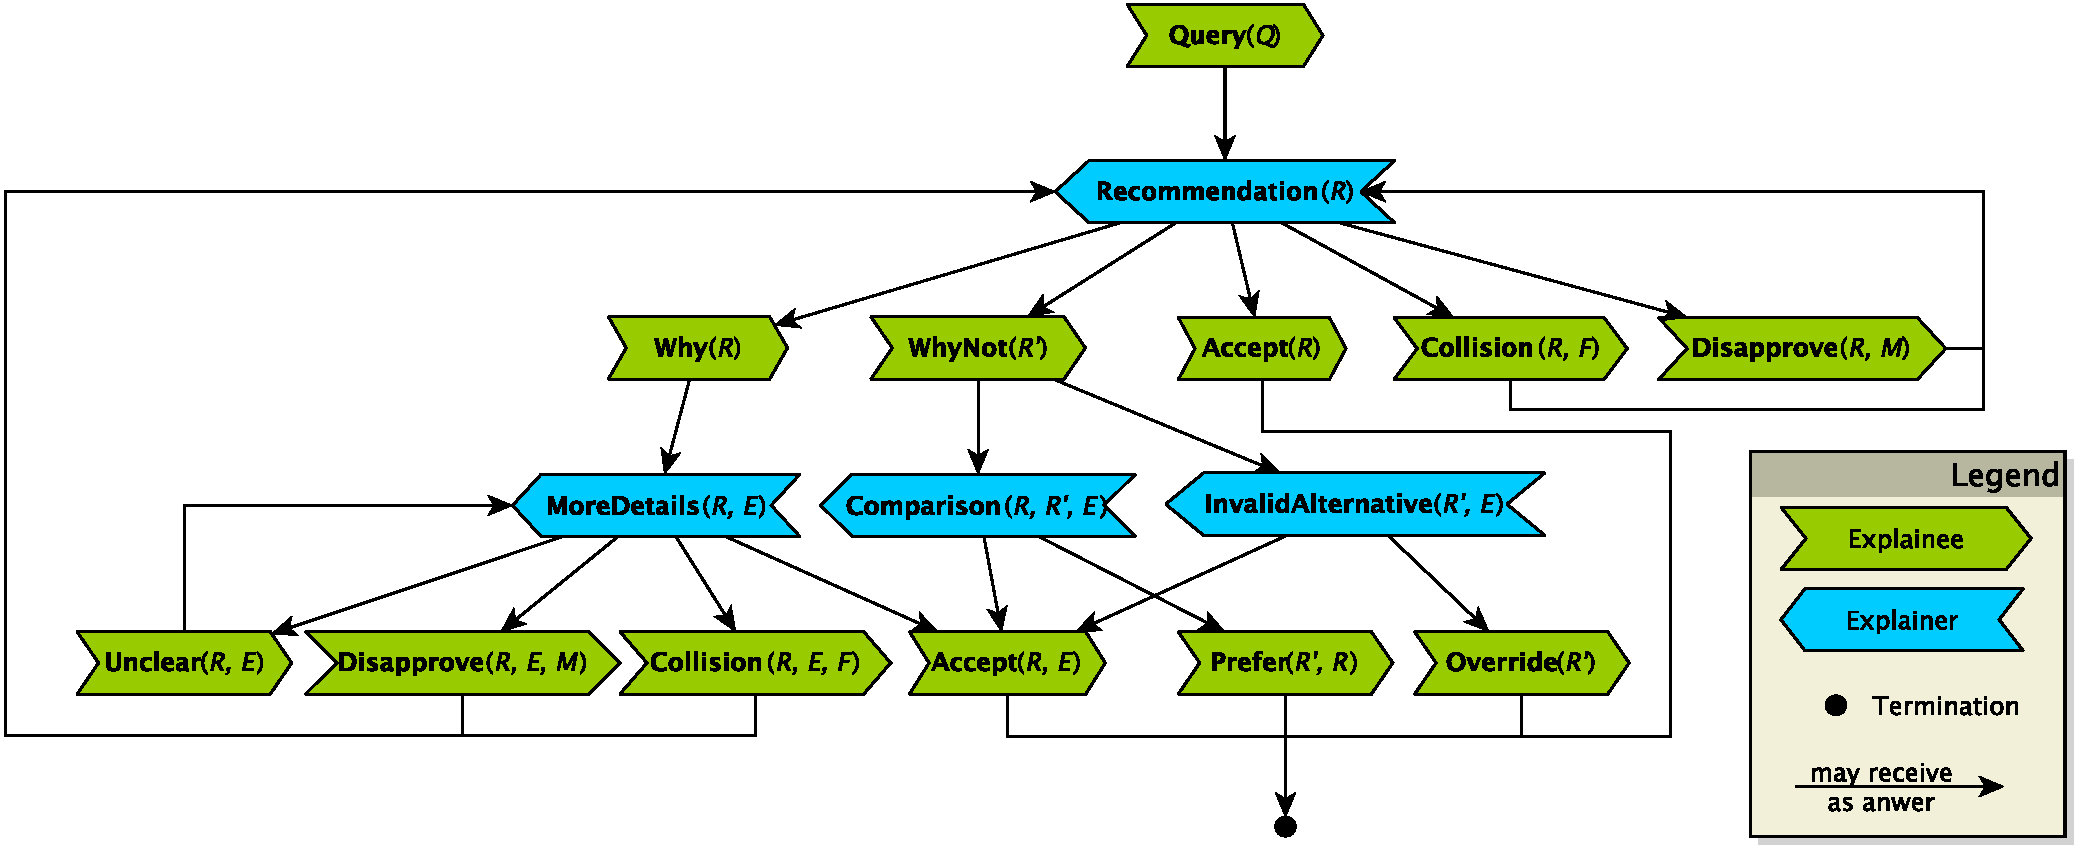
\includegraphics[width=\linewidth]{figures/pyxmas/user-agent-protocol}
    \caption{
      Message communication diagram between an explainer agent (blue boxes) and an explainee (green boxes).
      %
      Each box represents a message.
      %
      Arrows indicate the possible replies to each message.
    }
    \label{fig:protocol-messages}
\end{figure}
%
\Cref{fig:protocol-messages} presents an abstract formulation of the proposed protocol, which is independent of the specific representation or computation of recommendations and explanations.
%
The focus is on the exchange of messages between the explainer and the explainee, the information these messages carry, and the sequence in which they are exchanged.
%
The protocol defines two roles:
%
\begin{itemize}
    \item The explainee, who initiates the interaction.
    %
    \item The explainer, who responds to the explainee's queries.
\end{itemize}
%
Five data types are identified as the potential payloads exchanged during the protocol:
%
\begin{itemize}
    \item \textbf{Queries} (\(Q\)): Requests for recommendations submitted by the explainee.
    %
    \item \textbf{Recommendations} (\(R, R'\)): Responses to queries, provided by the explainer.
    %
    \item \textbf{Explanations} (\(E, E'\)): Information provided by the explainer to clarify recommendations.
    %
    \item \textbf{Features} (\(F\)): User-specific aspects that justify the rejection of a recommendation, which the explainer should consider in future interactions.
    %
    \item \textbf{Motivations} (\(M\)): Reasons for rejecting a recommendation, which may influence the explainer's behavior.
\end{itemize}
%
Thirteen message types are defined, each represented as a named record of the form \texttt{Name(Payload)}, where \texttt{Payload} consists of instances of the aforementioned data types.
%
Optional fields in the payload are denoted with a question mark.
%
The message types are summarized as follows:
%
\begin{enumerate}
    \item \texttt{Query(\(Q\))}: Sent by the explainee to initiate the protocol, carrying a recommendation request.
    %
    \item \texttt{Recommendation(\(Q, R\))}: Sent by the explainer in response to a query, carrying the query and the computed recommendation.
    %
    \item \texttt{Why(\(Q, R\))}: Sent by the explainee to request an explanation for a recommendation.
    %
    \item \texttt{WhyNot(\(Q, R, R'\))}: Sent by the explainee to request a contrastive explanation, comparing the recommendation with an alternative.
    %
    \item \texttt{Accept(\(Q, R, E?\))}: Sent by the explainee to accept a recommendation, optionally including the explanation.
    %
    \item \texttt{Collision(\(Q, R, F, E?\))}: Sent by the explainee to notify the explainer of a conflict between the recommendation and a personal feature.
    %
    \item \texttt{Disapprove(\(Q, R, M, E?\))}: Sent by the explainee to reject a recommendation, providing a reason and optionally the explanation.
    %
    \item \texttt{Details(\(Q, R, E\))}: Sent by the explainer to provide additional details about a recommendation.
    %
    \item \texttt{Comparison(\(Q, R, R', E\))}: Sent by the explainer to provide a contrastive explanation when the alternative recommendation is also valid.
    %
    \item \texttt{Invalid(\(Q, R', E\))}: Sent by the explainer to indicate that the alternative recommendation is invalid, with an explanation.
    %
    \item \texttt{Unclear(\(Q, R, E\))}: Sent by the explainee to indicate that the provided explanation is unclear.
    %
    \item \texttt{Prefer(\(Q, R, R'\))}: Sent by the explainee to express a preference for an alternative recommendation.
    %
    \item \texttt{Override(\(Q, R, R'\))}: Sent by the explainee to enforce an alternative recommendation, even if deemed invalid by the explainer.
\end{enumerate}
%
This abstract formulation ensures flexibility, allowing implementers to tailor the protocol to specific application domains.

Notably, messages are designed by keeping the \gls{ReST} [9] architectural style into account.
%
Hence, each message type is designed to carry all the information necessary for any involved party to decide which action to take next.
%
This is the reason why all/most messages carry the original query $Q$ and the recommendation $R$ (or $R'$) which they are referring to.
%
The message communication diagram from \Cref{fig:protocol-messages} depicts not only the messages exchanged by the explainee and explainer, but also the admissbile request–response patterns which the protocol allows.
%
There, a more detailed view of the message flow is provided, which we briefly summarise in the following.


\subsubsection{Relevant Scenarios and Protocol Analysis}\label{subsubsec:relevant-scenarios}
%
% !TeX spellcheck = en_GB
% !TeX root = ../phd-thesis.tex

\begin{figure}
    \centering{
        \begin{subfigure}[t]{0.4\linewidth}
            \centering
            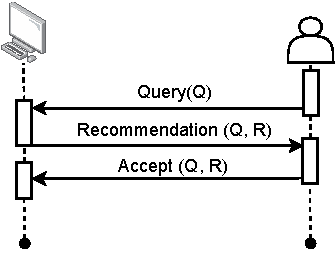
\includegraphics[width=\linewidth]{figures/quick-accept}
            \caption{Quick accept: the user accepts the recommendation without asking for explanations.}
            \label{fig:quick-accept}
        \end{subfigure}
        \hfill%\vline\hfill
        \begin{subfigure}[t]{0.4\linewidth}
            \centering
            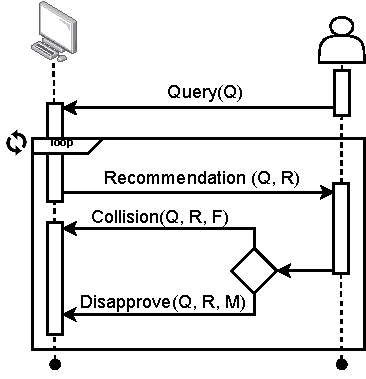
\includegraphics[width=\linewidth]{figures/quick-retry}
            \caption{Quick retry: the user rejects the recommendation without asking for explanations. Another recommendation is proposed, accordingly.}
            \label{fig:quick-retry}
        \end{subfigure}
    }

    \medskip

    \centering{
        \begin{subfigure}[t]{0.4\linewidth}
            \centering
            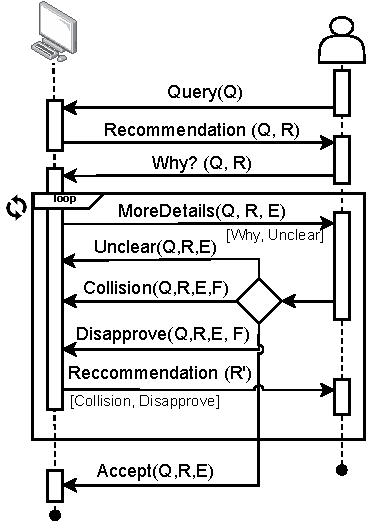
\includegraphics[width=\linewidth]{figures/explanation-loop}
            \caption{Ordinary explanation loop: the user asks `why' after a recommendation, and then agent answers with further details. The request for details may be repeated several times.}
            \label{fig:explanation-loop}
        \end{subfigure}
        \hfill%\vline\hfill
        \begin{subfigure}[t]{0.4\linewidth}
            \centering
            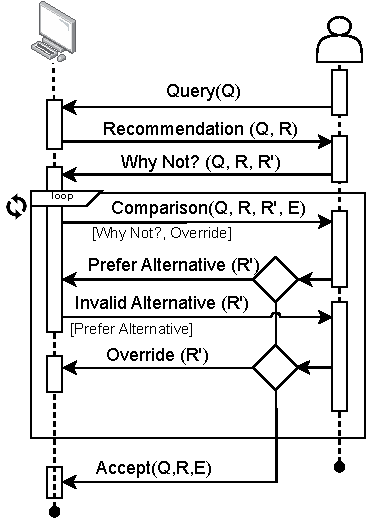
\includegraphics[width=\linewidth]{figures/contrastive-explanation-loop}
            \caption{Contrastive explanation loop: the user asks `why not' another recommendation. The agent may then explain why the other recommendation is acceptable or invalid. The user may either accept the original recommendation or prefer their own.}
            \label{fig:contrastive-explanation-loop}
        \end{subfigure}
    }
    \caption{Sequence diagrams describing most common scenarios of the protocol.}
    \label{fig:protocol-sequence-diagrams}
\end{figure}

%
The proposed protocol is versatile and accommodates various user needs and desires.
%
These include:
%
\begin{inlinelist}
    \item requesting a recommendation,
    \item seeking an explanation for the recommendation,
    \item asking for additional details about the explanation,
    \item simulating alternative recommendations, and
    \item providing feedback on recommendations or explanations.
\end{inlinelist}
%
\Cref{fig:protocol-sequence-diagrams} illustrates these scenarios, which are detailed below.

%
\paragraph{Quick Accept}
%
In this scenario, depicted in \Cref{fig:quick-accept}, the user accepts the recommendation without requiring an explanation.
%
For example, a user requests a restaurant recommendation, and the agent suggests a restaurant that the user finds satisfactory.

%
\paragraph{Quick Retry}
%
In \Cref{fig:quick-retry} the user rejects the recommendation without asking for an explanation.
%
The rejection may occur because the recommendation conflicts with the user's preferences or is unsuitable for the current context.
%
For instance, if the agent recommends a steakhouse to a vegetarian user, the user may signal a conflict with their preferences.
%
Alternatively, the user may simply disapprove of the recommendation without providing specific feedback.
%
In both cases, the agent generates a new recommendation.
%
The agent is expected to learn from conflicts but not from generic disapprovals.

%
\paragraph{Ordinary Explanation Loop}
%
In the case shown in \Cref{fig:explanation-loop}, the user requests an explanation for the recommendation.
%
If the explanation is unsatisfactory, the user may ask for further details, initiating an iterative process.
%
This loop continues until the user either accepts the recommendation or requests a new one.
%
The protocol supports ``zooming'' explanations, where the agent adjusts the granularity of the explanation.
%
For example, the agent may first provide local explanations, describing how the specific recommendation was generated.
%
Subsequently, it may offer global explanations, detailing the general logic behind its recommendations.
%
The agent can also switch between textual and visual explanations to enhance clarity.
%
Consider a user who requests a restaurant recommendation.
%
The agent suggests an Asian restaurant with a high rating and proximity to the user.
%
If the user asks for an explanation, the agent may state that the restaurant matches the user's taste for sushi and is within 1 km.
%
If further details are requested, the agent may explain its general recommendation strategy, such as prioritizing highly rated restaurants within a certain distance.

%
\paragraph{Contrastive Explanation Loop}
%
Lastly, in \Cref{fig:contrastive-explanation-loop}, the user requests a contrastive explanation, comparing the given recommendation \(R\) with an alternative \(R'\).
%
If \(R'\) is valid, the agent provides a comparison, highlighting why one recommendation is preferable.
%
If \(R'\) is invalid, the agent explains why it cannot be recommended.
%
The user may then accept the original recommendation, prefer the alternative, or override the agent's decision.
%
For example, if the agent recommends an Asian restaurant, but the user prefers a steakhouse, the agent may compare the two options.
%
If the steakhouse aligns with the user's dietary goals, the agent may note that the Asian restaurant is closer.
%
If the steakhouse violates dietary goals, the agent explains this conflict.
%
In either case, the user decides whether to accept the original recommendation or override it.
%
The agent learns from overrides to refine future recommendations.


\subsubsection{Which Sorts of Explanations and Recommendations?}
\label{subsubsec:which-sorts-of-explanations-and-recommendations}

The proposed explanation protocol is agnostic regarding the specific representation of explanations and recommendations.
%
It is the responsibility of the implementer to define how explanations and recommendations are represented and computed.
%
The protocol only specifies \emph{when} these elements should be computed.

\Glspl{RS} typically rely on one or more \gls{ML} predictors trained on user data.
%
Whether the training of these predictors is performed by the recommender agent or if the agent is equipped with pre-trained predictors at deployment is an implementation detail.
%
In either case, the recommender agent must have access to user profile information.
%
This information can be obtained during an initial configuration phase or inferred from user interactions, such as accepted or rejected recommendations.
%
To support dynamic learning, the agent should include a learning algorithm capable of updating the predictors when new user data becomes available.
%
From this perspective, the explainer agent acts as a proxy for the \gls{ML} predictor(s).

Explanations, however, are not necessarily derived from \gls{ML} predictors.
%
The \gls{XAI} literature offers a wide range of approaches for generating explanations, including visual, textual, and numerical methods~\cite{BarredoArrieta2020,DBLP:journals/csur/GuidottiMRTGP19,DBLP:journals/csur/CiattoSAMO24}.
%
The explainer agent must not only wrap the \gls{ML} predictor(s) but also encapsulate the logic for computing and representing explanations.

A critical challenge arises when recommendations and explanations use different representation formats, such as textual and visual.
%
In such cases, the explainer agent must bridge the gap by providing a unified representation of both the recommendation and its explanation.
%
To address this, designers may consider adopting computational logic as a unifying framework for recommendations and explanations.
%
In computational logic, both knowledge bases and queries are represented as logic formulas.
%
These formulas can be used to represent recommendation requests, solutions, and explanations.

For example, a recommendation query can be expressed as the logic goal:
%
\[
\texttt{should\_eat(Food, lunch)},
\]
%
where \texttt{Food} is a logic variable representing an unknown value.
%
Recommendations, such as \( R, R', R'' \), correspond to logic solutions, e.g., \(\texttt{Food} = \texttt{paella}\).
%
Explanations \( E, E', E'' \) can take various forms:
%
\begin{itemize}
    \item \textbf{Local explanations:} The path in the proof tree computed by the explainer agent to derive the recommendation.
    %
    \item \textbf{Global explanations:} The logic program used by the explainer agent to generate the recommendation.
    %
    \item \textbf{Contrastive explanations:} Metrics comparing multiple recommendations or identifying constraints that make certain recommendations invalid.
    %
    \item \textbf{Combinations:} Any combination of the above types.
\end{itemize}

User features, such as \( F, F', F'' \), may include raw facts describing the user, e.g., \texttt{age(31)}, \texttt{goal(lose\_weight)}, or \texttt{category(vegetarian)}.
%
Motivations for disapproval can include predefined facts, such as:
%
\begin{itemize}
    \item \texttt{dislike:} The user dislikes the recommendation, prompting the agent to learn from this feedback.
    %
    \item \texttt{not\_now:} The user does not want the recommendation at the moment, but may accept it in the future. In this case, the agent should not memorize the rejection.
\end{itemize}


\subsection{From Theory to Practice with \textsc{PyXMas}}
\label{subsec:from-theory-to-practice-with-pyxmas}
%
\begin{figure}
    \centering
    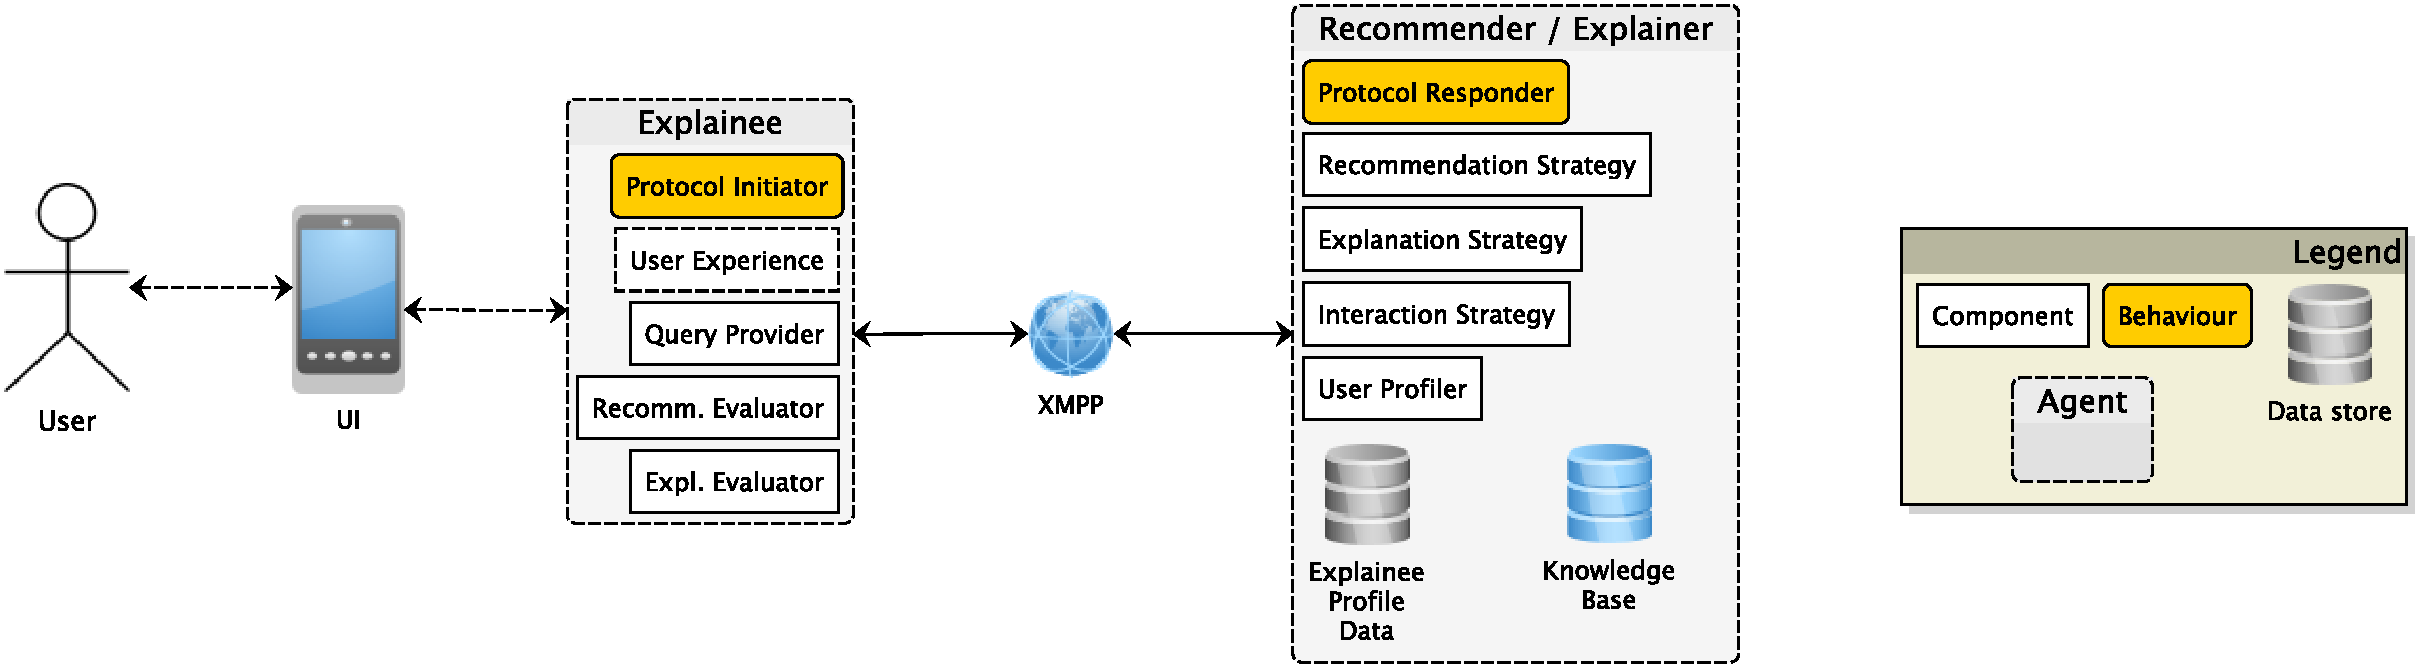
\includegraphics[width=\linewidth]{figures/pyxmas/architecture}
    \caption{
        Modular architecture of \textsc{PyXMas}.
        %
        The library provides parametric behaviours that can be customized by implementing specific components.
        %
        If the explainee agent is human, a UX component may be required to facilitate interaction via a device.
    }
    \label{fig:architecture}
\end{figure}
%
This section describes how the proposed protocol can be implemented as agent-oriented software.
%
We introduce \textsc{PyXMas}\footnote{\url{https://github.com/pikalab-unibo/pyxmas}}, a Python library for explainable multi-agent systems (\glspl{MAS}).
%
The library is built on \textsc{Spade} and provides reusable implementations of the protocol described in \Cref{subsec:abstract-formulation-of-the-protocol}.
%
This allows researchers and developers to focus on designing recommender and explainer agents, as well as defining the representation of recommendations and explanations, without re-implementing the protocol.


\subsubsection{\textsc{PyXMas} Architecture}
\label{subsubsec:pyxmas-architecture}
%
\Cref{fig:architecture} illustrates the modular architecture of \textsc{PyXMas}.
%
The library defines two main behaviours:
%
\begin{inlinelist}
    \item the \emph{initiator}, responsible for sending recommendation queries and processing responses, and
    %
    \item the \emph{responder}, responsible for computing and returning recommendations and explanations.
\end{inlinelist}
%
The initiator behaviour is designed for the explainee agent, while the responder behaviour is intended for the explainer agent.
%
Both behaviours are parametric, allowing users to customize their functionality by implementing specific components.

\paragraph{Explainer Agent}
%
The explainer agent requires the following components:
%
\begin{itemize}
    \item \textbf{Recommendation Strategy:} Computes recommendations based on user queries, preferences, and goals (e.g., ``vegetarian'' or ``weight loss'').
    %
    The strategy can adapt over time by learning from user feedback.
    %
    \item \textbf{Explanation Strategy:} Generates explanations for recommendations, leveraging user profiles and domain knowledge (e.g., ``ingredient X is plant-based'').
    %
    \item \textbf{User Profiler:} Learns user preferences from feedback using heuristic or \gls{ML}-based methods.
    %
    This enables the agent to refine recommendations and explanations dynamically.
    %
    \item \textbf{Interaction Strategy:} Manages how recommendations and explanations are presented to the explainee.
    %
    For example, a humanoid robot may use gestures or facial expressions to enhance interaction.
\end{itemize}
%
The explainer agent stores two types of data:
%
\begin{inlinelist}
    \item user profile data, and
    %
    \item domain knowledge.
\end{inlinelist}
%
These are maintained in dedicated data stores and updated as needed.

\paragraph{Explainee Agent}
%
The explainee agent requires the following components:
%
\begin{itemize}
    \item \textbf{Query Provider:} Generates queries based on the explainee's goals.
    %
    \item \textbf{Recommendation Evaluator:} Assesses recommendations and decides whether to accept or reject them.
    %
    \item \textbf{Explanation Evaluator:} Evaluates explanations and influences the recommendation evaluator accordingly.
\end{itemize}
%
If the explainee is a human user, the agent acts as a proxy, mediating interactions via a \gls{UI} on a device (e.g., a smartphone).
%
In this case, a \textbf{\gls{UX}} component is required to manage the \gls{UI}, process user inputs, and present recommendations and explanations.


\subsubsection{PyXMas Design}\label{subsubsec:pyxmas-design}
%
\begin{figure}
    \centering
    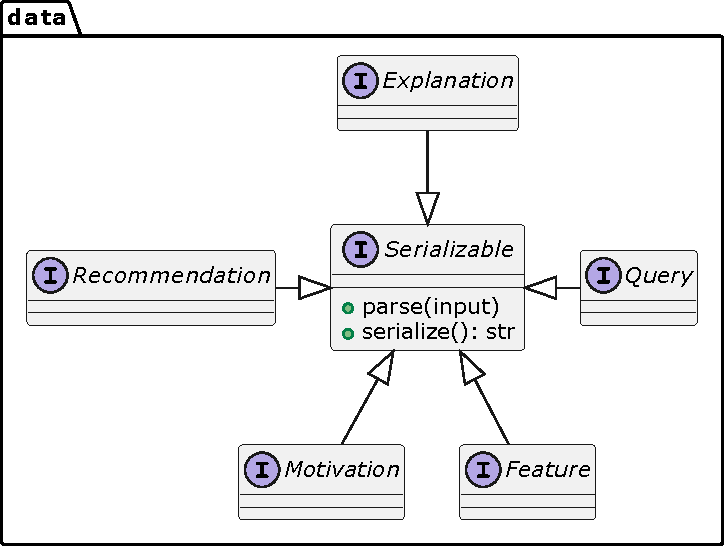
\includegraphics[width=0.7\linewidth]{figures/pyxmas/types}
    \caption{
        Abstract classes for message payloads in \textsc{PyXMas}.
    }
    \label{fig:types}
\end{figure}
%
\textsc{PyXMas} is a Python library designed for developing explainable \glspl{MAS}.
%
It provides:
%
\begin{itemize}
    \item Abstract classes for the (de)serialization of message payloads exchanged between the explainer and explainee agents (see \Cref{fig:types}).
    %
    \item Abstract classes defining the initiator and responder behaviors.
\end{itemize}
%
These abstract classes allow developers to extend and customize their functionality by overriding specific methods.
%
This flexibility enables the creation of tailored explainable \glspl{MAS}.
%
\paragraph{Data Types for Message Payloads}
%
As illustrated in \Cref{fig:types}, \textsc{PyXMas} provides five abstract classes corresponding to the data types defined in \Cref{subsec:abstract-formulation-of-the-protocol}.
%
These classes enforce serialization, ensuring that data can be converted to and from strings.
%
This is essential for enabling communication between the explainer and explainee agents over the network.
%
Developers can define custom representations for queries, recommendations, explanations, and other data types by extending these abstract classes.
%
The only requirement is that the serialized data must be both machine- and human-readable.
%
\paragraph{Predefined Behaviors}
%
\begin{figure}
    \centering
    \begin{subfigure}[t]{\linewidth}
        \centering
        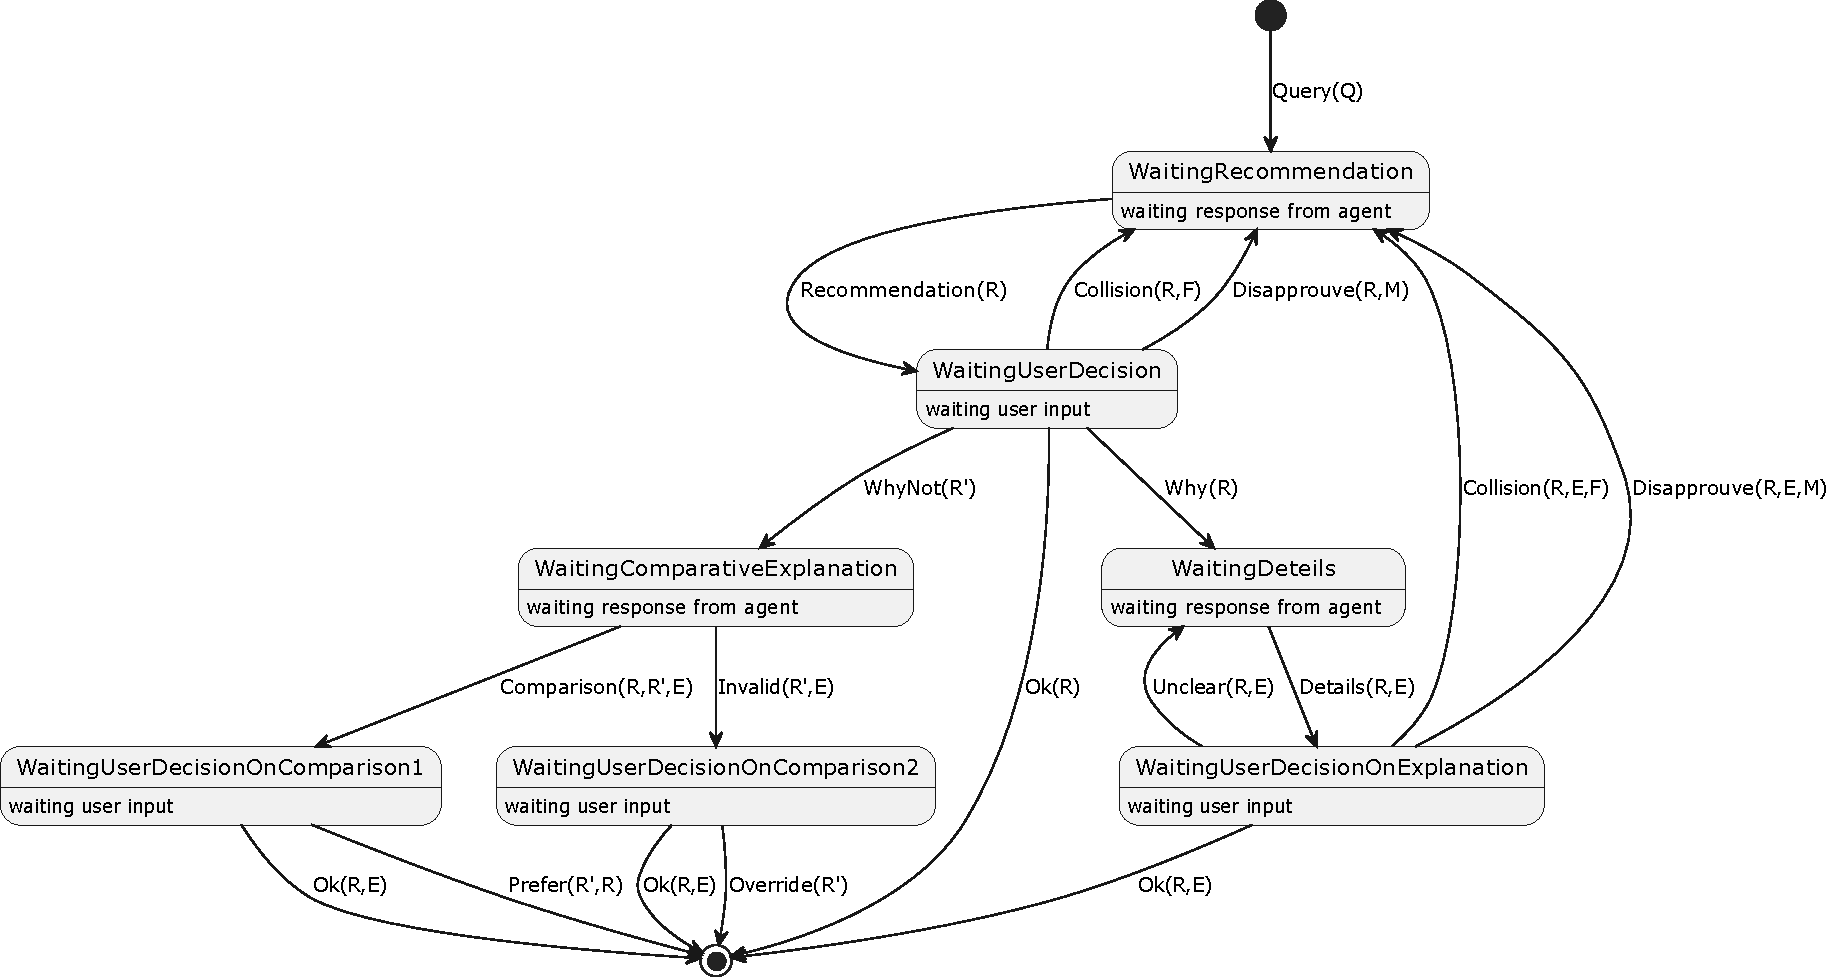
\includegraphics[width=\linewidth]{figures/pyxmas/user-state-diagram}
        \caption{
            Initiator-side state diagram.
        }
        \label{fig:user-state-diagram}
    \end{subfigure}
    %
    \begin{subfigure}[t]{\linewidth}
        \centering
        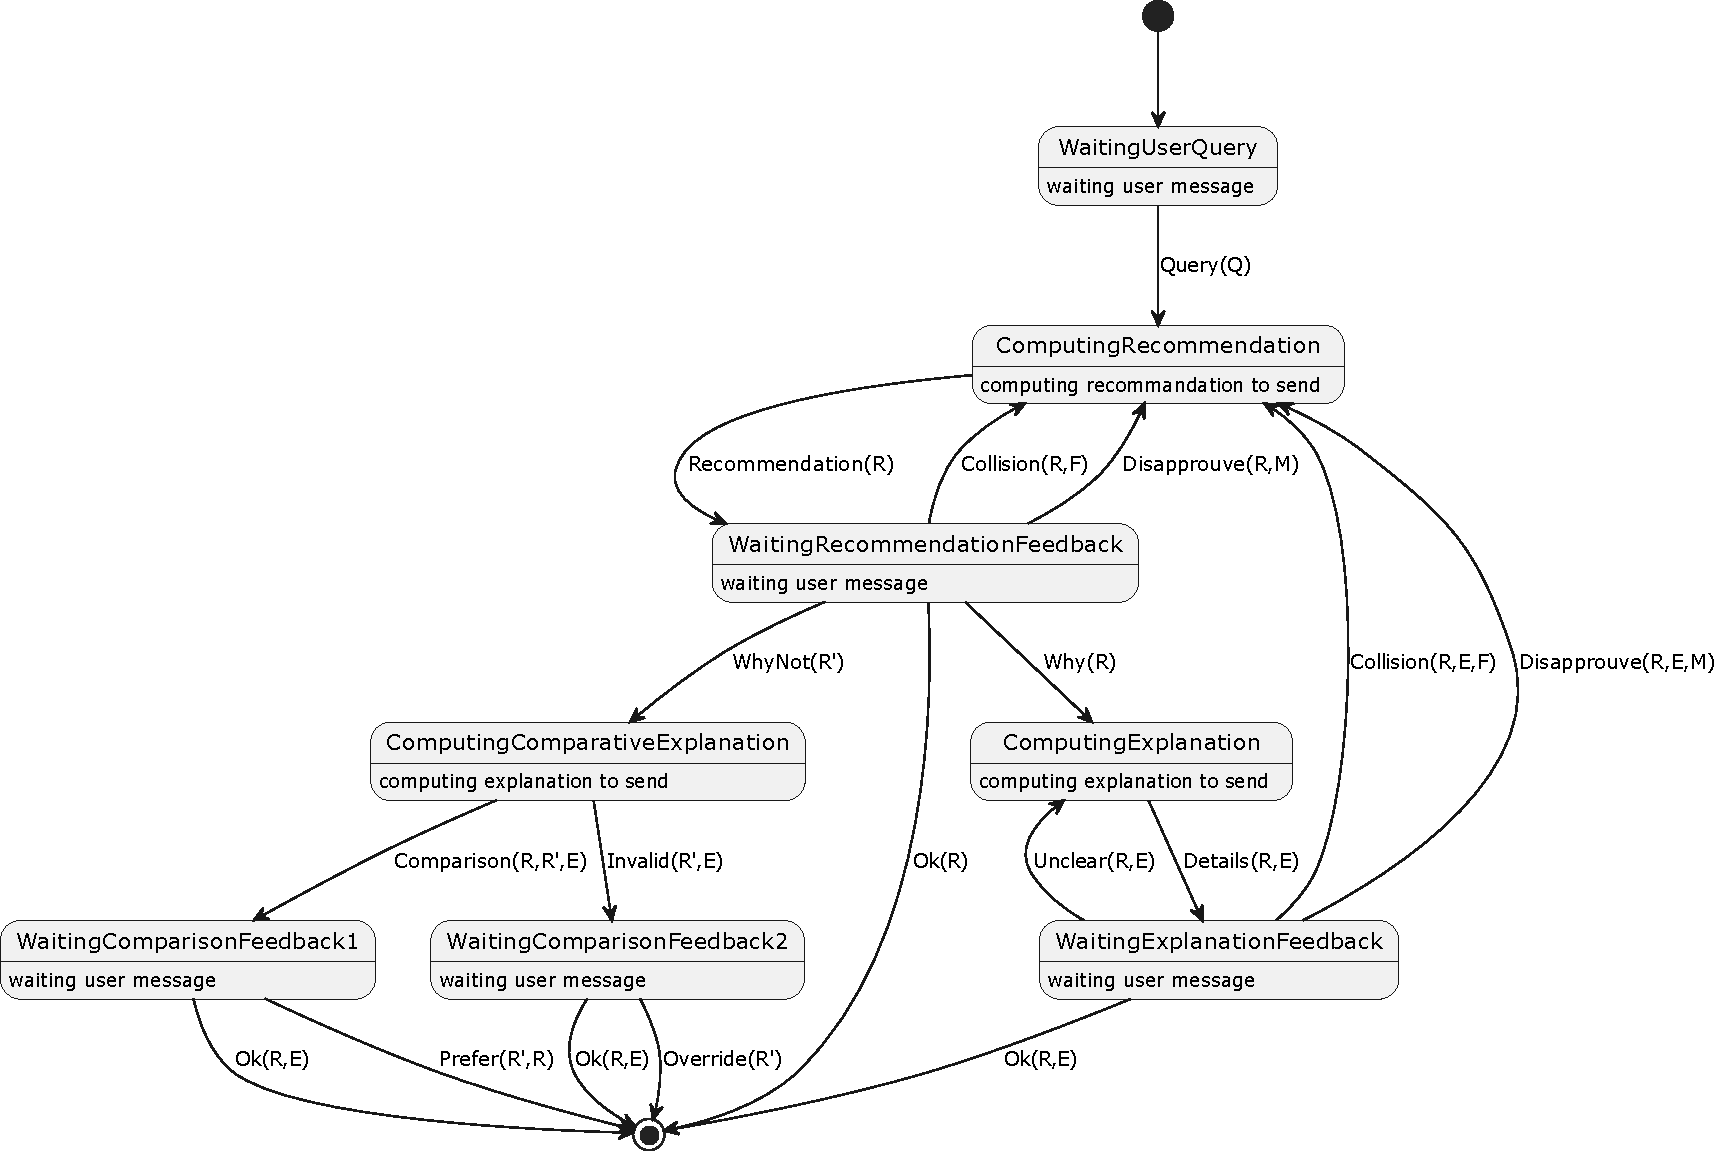
\includegraphics[width=\linewidth]{figures/pyxmas/agent-state-diagram}
        \caption{
            Responder-side state diagram.
        }
        \label{fig:agent-state-diagram}
    \end{subfigure}
    \caption{
        State diagrams describing the initiator and responder behaviors in \textsc{PyXMas}.
    }
    \label{fig:state-diagrams}
\end{figure}
%
\textsc{PyXMas} provides two abstract classes for the protocol roles:
%
\begin{itemize}
    \item The \emph{initiator}, which represents the explainee agent.
    %
    \item The \emph{responder}, which represents the explainer agent.
\end{itemize}
%
These behaviors are implemented as finite-state machines (FSMs) using \textsc{Spade}.
%
Each state corresponds to a specific action, such as waiting for a message or processing a response.
%
\Cref{fig:state-diagrams} illustrates the state diagrams for the initiator and responder behaviors.
%
On the initiator side, developers can override callbacks to control:
%
\begin{itemize}
    \item Query generation.
    %
    \item Evaluation of recommendations and decisions to accept or reject them.
    %
    \item Evaluation of explanations and their influence on recommendation acceptance.
\end{itemize}
%
On the responder side, developers can override callbacks to control:
%
\begin{itemize}
    \item Recommendation generation.
    %
    \item Explanation generation.
    %
    \item Handling of accepted or rejected recommendations.
\end{itemize}
%
This design ensures that \textsc{PyXMas} can be adapted to various application domains while maintaining a clear and modular structure.



\section{NeSy \Gls{AI} for supporting chronic disease diagnosis and monitoring}\label{sec:nesy-ai-for-supporting-chronic-disease-diagnosis-and-monitoring}

%\subsection{\Gls{LLM}-based solutions for healthcare chatbots: a comparative analysis}\label{subsec:llm-based-solutions-for-healthcare-chatbots-a-comparative-analysis}

%\subsection{Open-source small language models for personal medical assistant chatbots}\label{subsec:open-source-small-language-models-for-personal-medical-assistant-chatbots}

\section{Applying \Gls{RAG} on open \Glspl{LLM} for a medical chatbot supporting hypertensive patients}\label{sec:applying-rag-on-open-llm-for-a-medical-chatbot-supporting-hypertensive-patients}